%\documentclass[aps,prd,nofootinbib]{revtex4-1}
\documentclass[singlepage,notitlepage,nofootinbib,11pt]{revtex4-1}
\usepackage{amsmath}
\usepackage{graphicx}
\usepackage{subfig}
\usepackage{epsfig}
\usepackage{listings}
\usepackage[hidelinks,hyperfootnotes=false,bookmarks=false,colorlinks=true]{hyperref}

\newcommand{\eq}[1]{\begin{align*}#1\end{align*}}
\newcommand{\pmat}[1]{\begin{pmatrix}#1\end{pmatrix}}
\newcommand{\center}[1]{\begin{center}#1\end{center}}
\def\<{\langle}
\def\>{\rangle}
\def\l{\left}
\def\r{\right}


\begin{document}
\title{Problem Set 5 - G6080}
\author{Victor Genty}
\email{vgenty@nevis.columbia.edu}
\homepage{www.nevis.columbia.edu/~vgenty}
\date{\today}
\begin{abstract}
\centering
Source code can be found at \href{https://github.com/vgenty/G6080/tree/master/ps5}{github.com/vgenty/G6080/ps5}
\end{abstract}
\maketitle
\section{Poisson's Equations}
I implemented the conjugate gradient method in \texttt{poissonONE.cpp} to solve poisson's equation for the given charge and boundary conditions. I used the C++ library \texttt{eigen3} which is a template library for linear algebra: matricies, vectors, numerical solvers, and related algorithms. After the completion of the program for the specified lattice spacing the potential is written to a \texttt{ROOT} file and plotted in \texttt{plotter.py}, a python script. For the first part I chose two different nearby locations and computed $V(x,y)$ for a few lattice spacing to see if the points appeared to converge to some value. I think fit a linear function to the data points to extrapolate to zero lattice spacing. The results are plotted in Fig. \ref{extrapolation}. For smaller lattice spacing $a$ the potential appeared to get {\it closer} together signifying a convergence to a true ``continuous'' value. The extrapolation to zero $a$ (the y-intercept) is shown for each of the two plots.  The two calculation of potential are near eachother and should therefore have nearly equivalent y-intercepts with the small deviation being attributed to the change in potential. This is clearly the case. We now plot the potential distribution as a surface plot in \texttt{ROOT}. The salient features of Fig. \ref{poissons} are zero boundary conditions at the edges, a negative point charged situated south of the constant positive potential plateau, and a region of fixed positive potential. In the continuous case the negative charge is considered as a dirac delta function at the point in question, this is not possible for discrete case. To avoid this I smeared out the charge onto the four nearby lattice points creating an effective surface charge rather than a point charge. For smaller and smaller lattice spacing the surface charge will mimick a point of infinite potential. The physical shape of the result in Fig. \red{poissons} is as expected for a solution to the boundary value problem.
\begin{figure}[h]
  \centering
  \captionsetup[subfigure]{labelformat=empty}
  \subfloat[][]{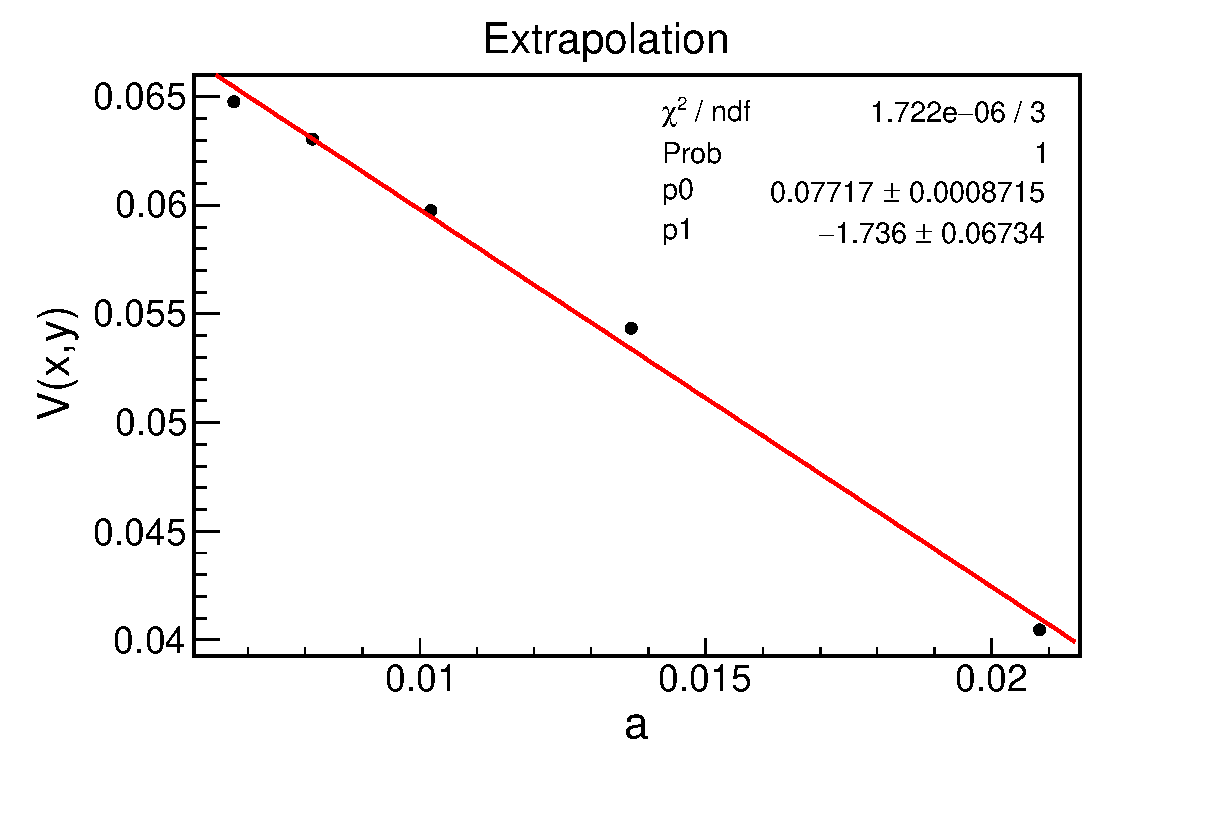
\includegraphics[width=0.5\textwidth]{figures/ex1.eps}}
  \subfloat[][]{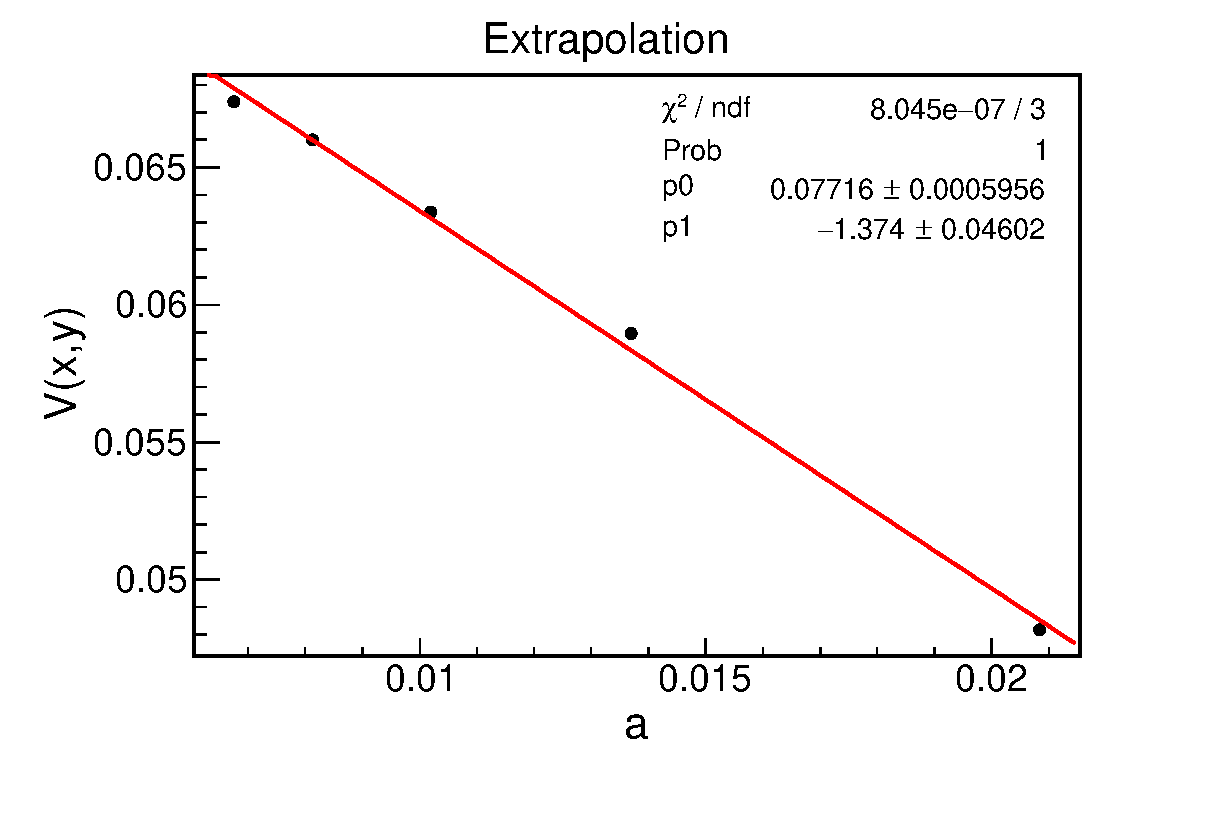
\includegraphics[width=0.5\textwidth]{figures/ex2.eps}}
  \caption{\label{extrapolation} Extrapolation of the grid spacing to zero $a$ for two nearby points on the the 2D grid. The fit parameters are shown in the top right of each plot. The variable p0 shows the y-intercept and $a=0$ extrapolation.}
\end{figure}
\begin{figure}[h]
  \centering
  \captionsetup[subfigure]{labelformat=empty}
  \subfloat[][]{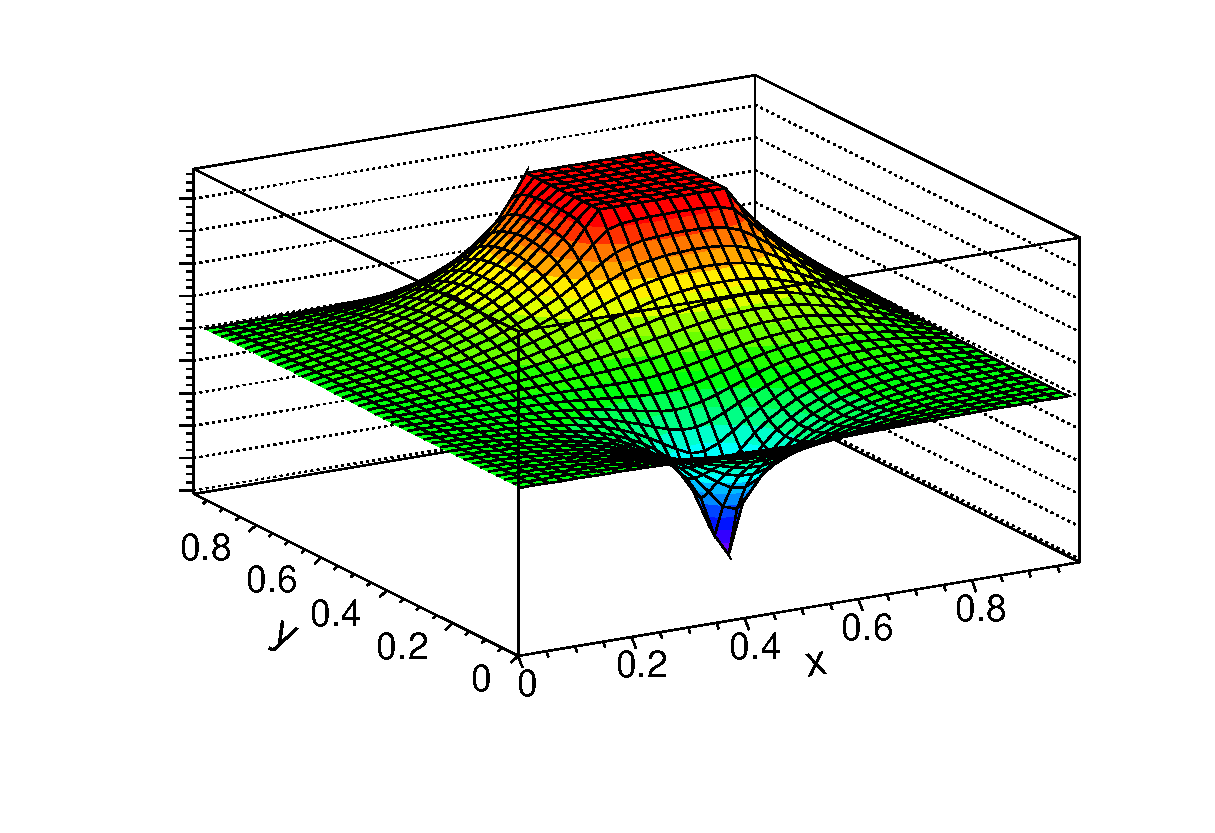
\includegraphics[width=0.5\textwidth]{figures/poisson.eps}}
  \subfloat[][]{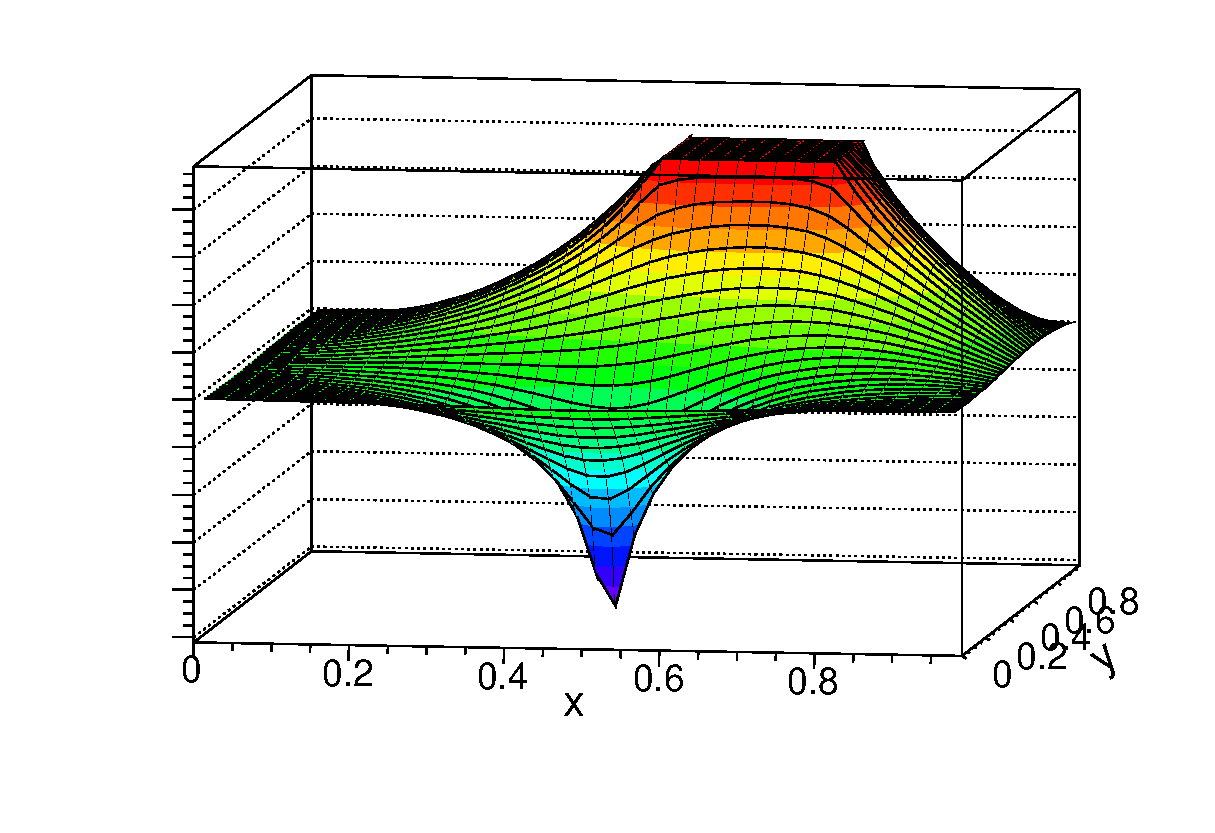
\includegraphics[width=0.5\textwidth]{figures/poisson2.eps}}\\
  \subfloat[][]{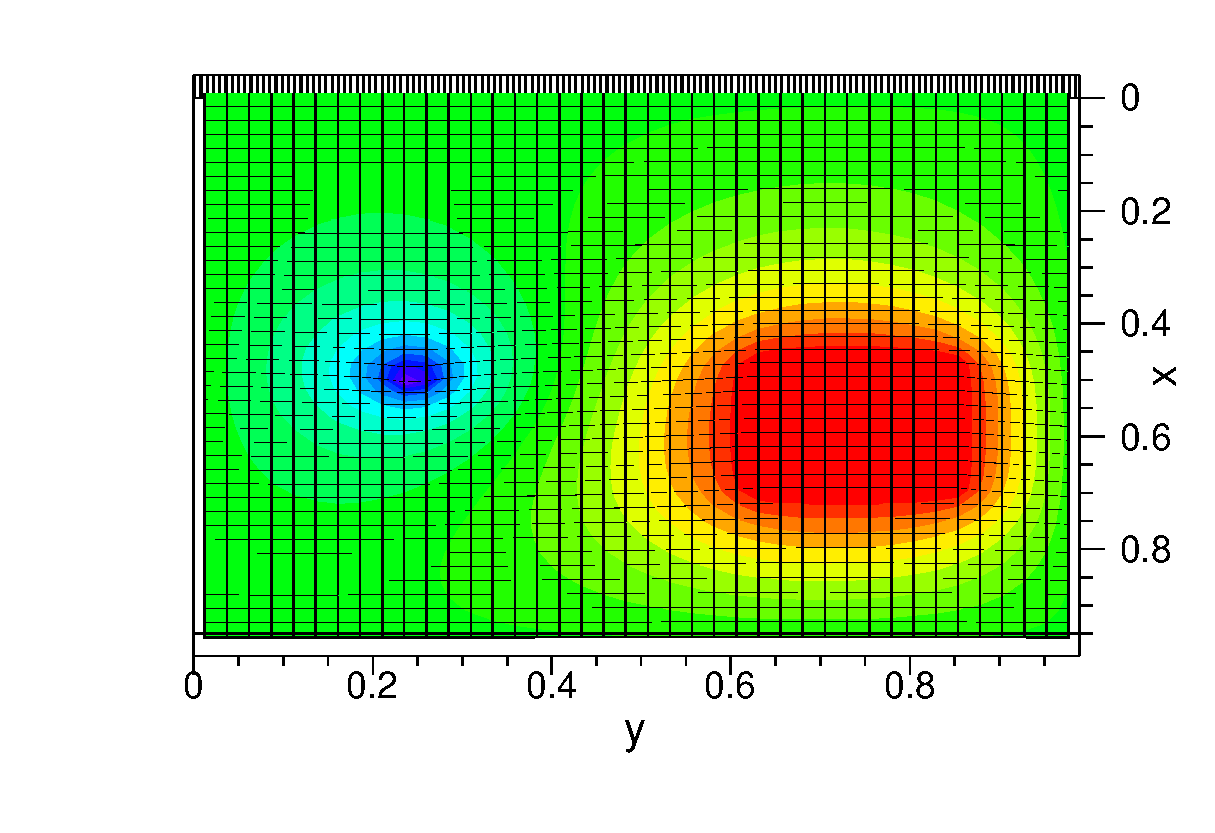
\includegraphics[width=0.5\textwidth]{figures/poisson3.eps}}
  \subfloat[][]{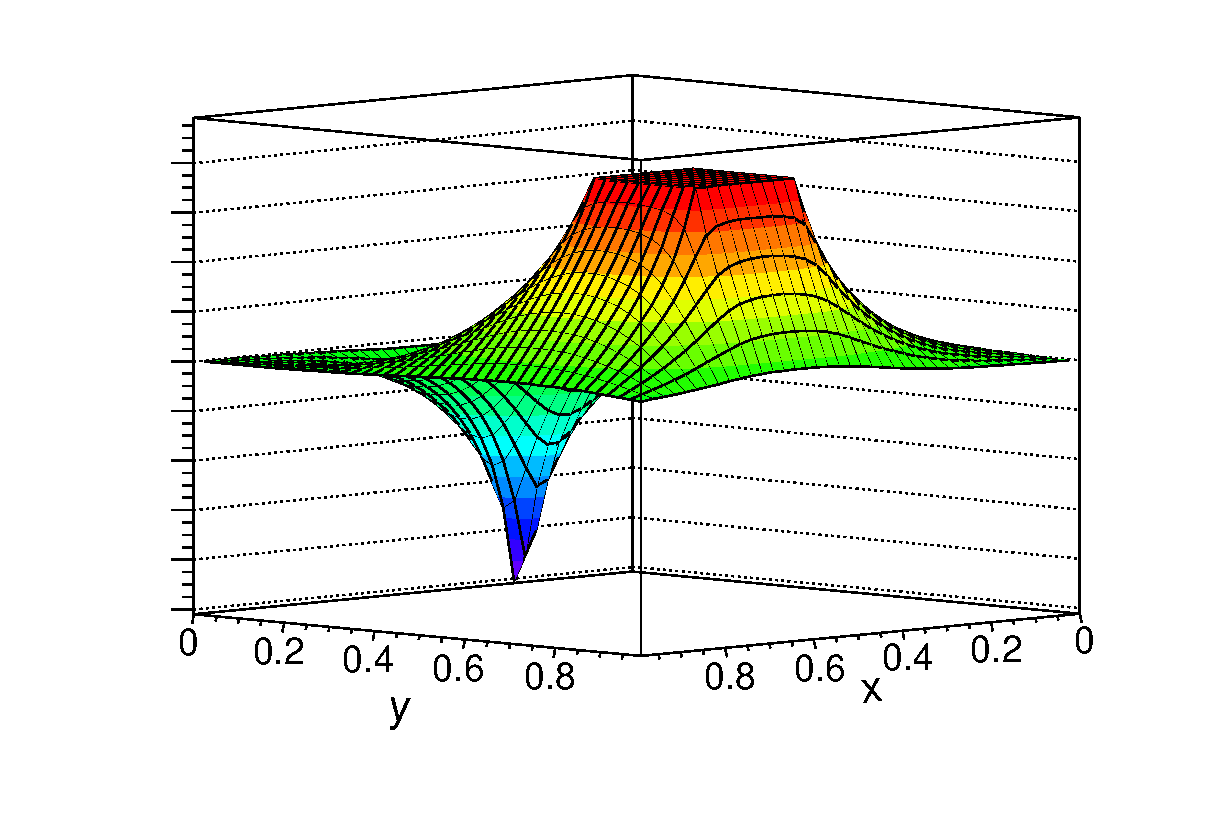
\includegraphics[width=0.5\textwidth]{figures/poisson4.eps}}
  \caption{\label{poissons} ``SURF'' plot for 2D discrete poisson solver with grid size $a\sim0.01$. Four different views are shown. The deep blue color is most negative, red being the largest, and green representing zero.}
\end{figure}
\clearpage

\section{Free particle Schrodinger equation}
We now consider the quantum mechanics of an uncharged particle bounded in the same square region with the point charge removed. Here we let the mass of the particle be $m=1/10$ in dimensionless units ($\hbar = 1$). The boundary and internal rectangle are infinite potential (where the particle wavefuntion must vanish). I implemented the invserse iteration scheme to find the three lowest eigenvalues of the energy satisfying the equation,
\begin{align*}
  -\frac{1}{2m} \nabla^2\psi + V(x,y)\psi = E\psi.
\end{align*}
The results for the three lowest probability distributions for the particle in the box with lattice spacing $a\sim0.01$ are shown in Fig. \ref{particles}. The three lowest eigen-energies to three significant figures are in the table below.
\begin{center}
  \begin{tabular}{ c | c | c | c }
    \hspace{1pt} & Ground & 1$^{\text{st}}$ excited & 2$^{\text{nd}}$ excited \\ \hline
    Energy & 151 & 270 & 368
    \end{tabular}
\end{center}
The particle in the box resembles the unperturbed harmonic solution to the 2 dimensional square well with the particle avoiding the rectagular region, because of this the energy does not scale as $n^2$ (the square of the numer of anti-nodes). The probability distribution does show the expected increase in number of nodes the higher the energy where is it is more probable on average to be found in a larger region of the box (spreading out).
\begin{figure}[h]
  \centering
  \captionsetup[subfigure]{labelformat=empty}
  \subfloat[][]{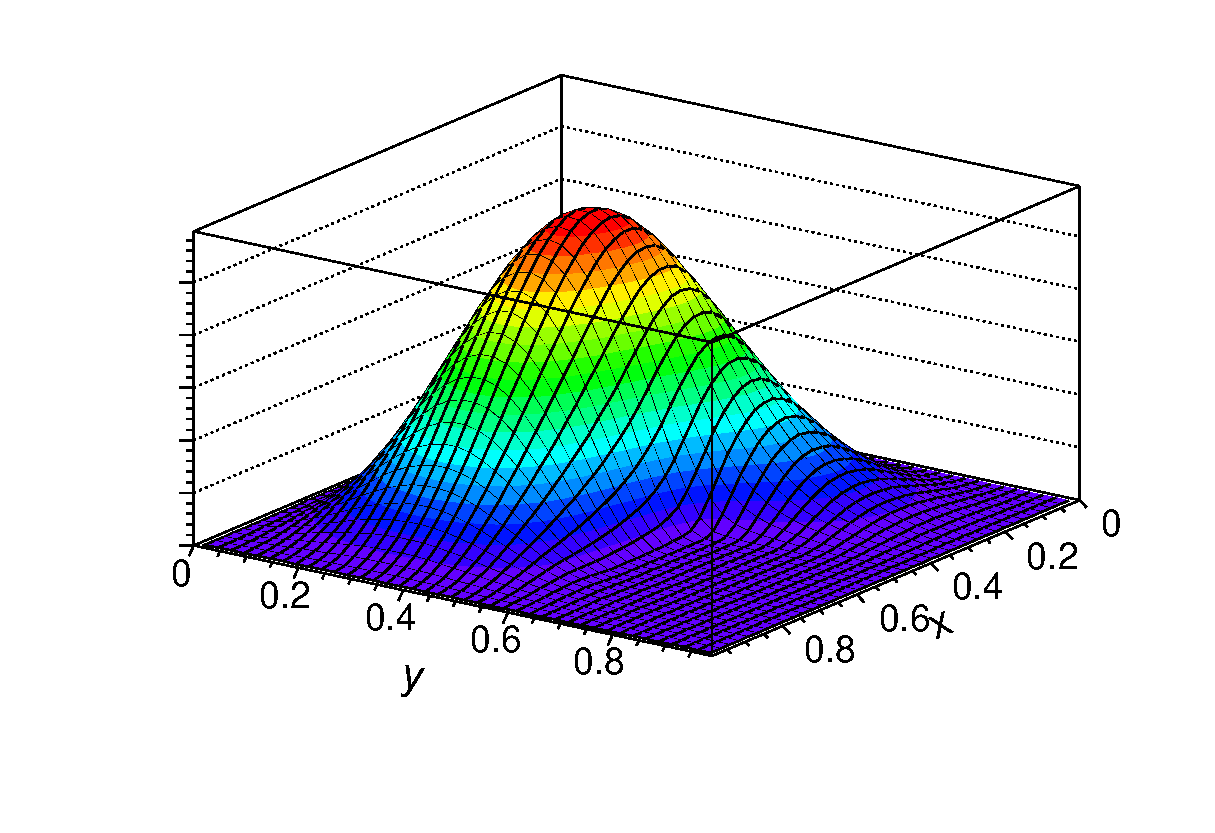
\includegraphics[width=0.5\textwidth]{figures/lowest1.eps}}
  \subfloat[][]{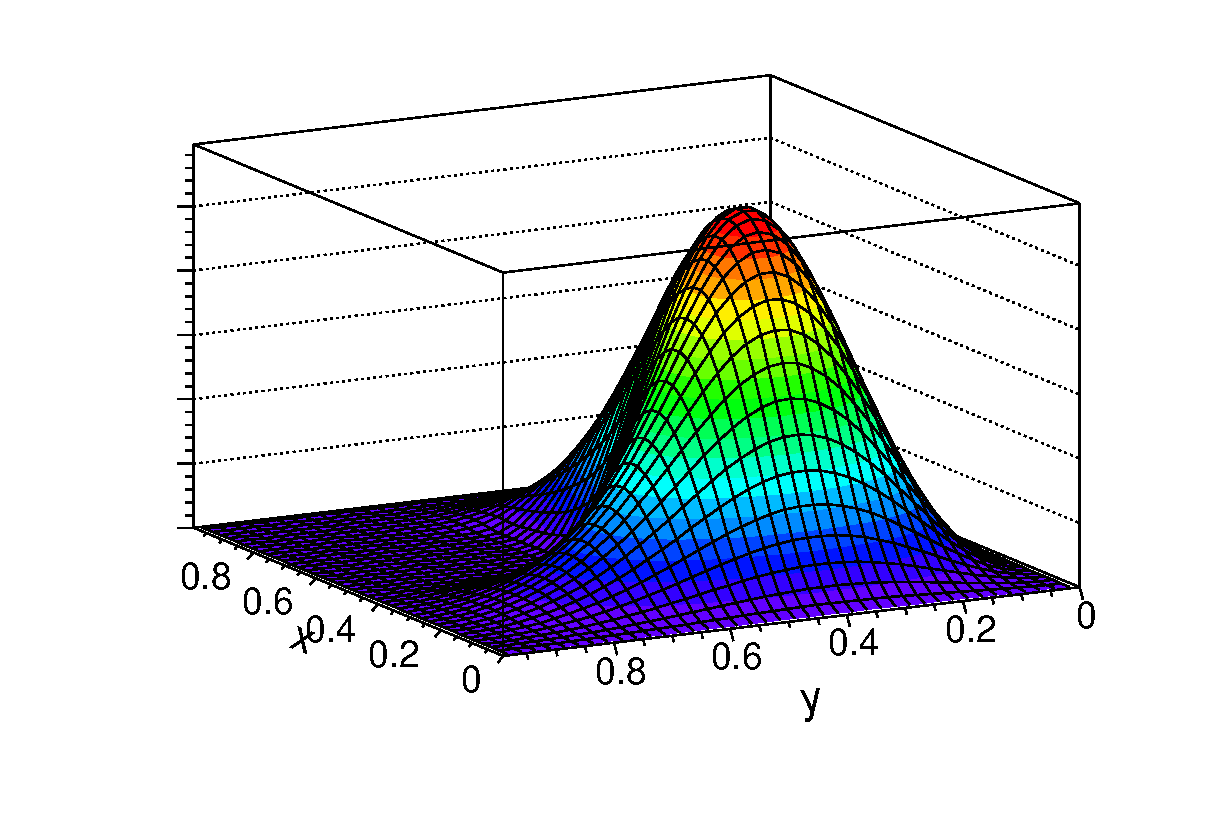
\includegraphics[width=0.5\textwidth]{figures/lowest2.eps}}\\
  \subfloat[][]{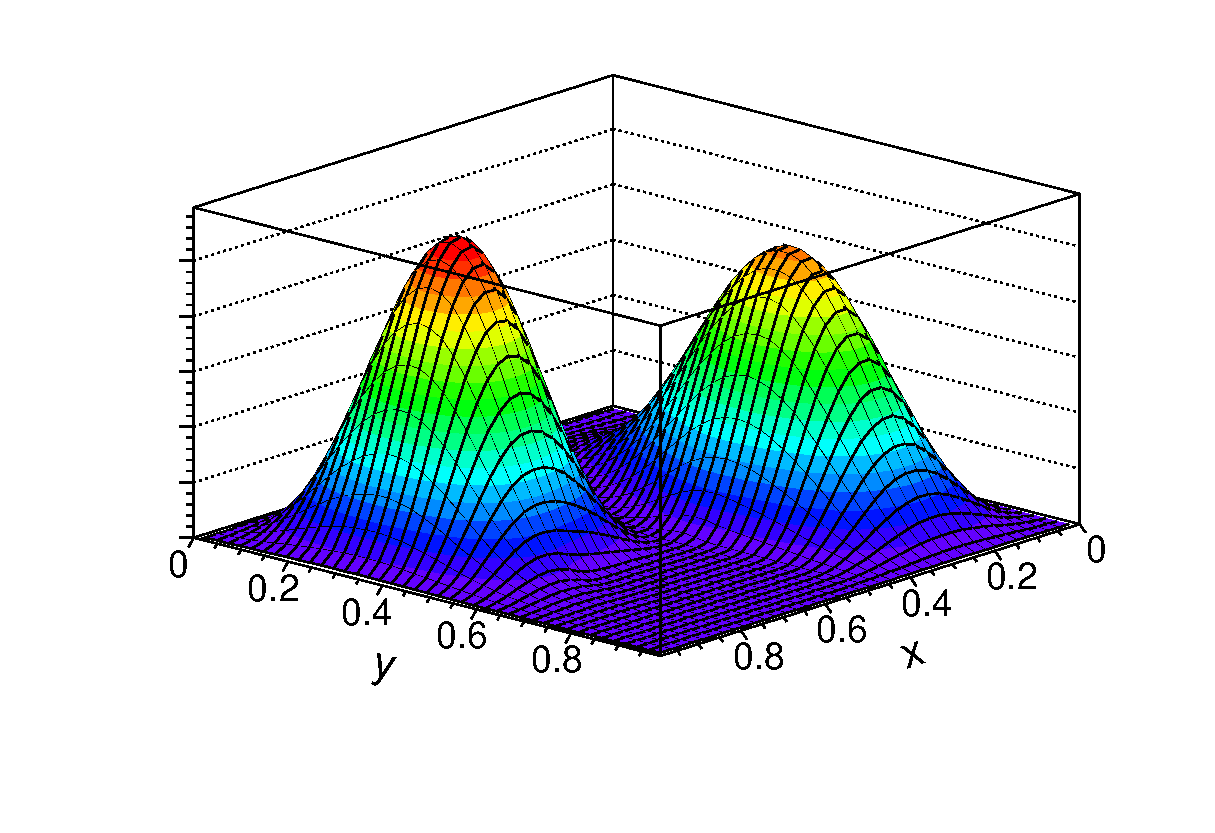
\includegraphics[width=0.5\textwidth]{figures/second1.eps}}
  \subfloat[][]{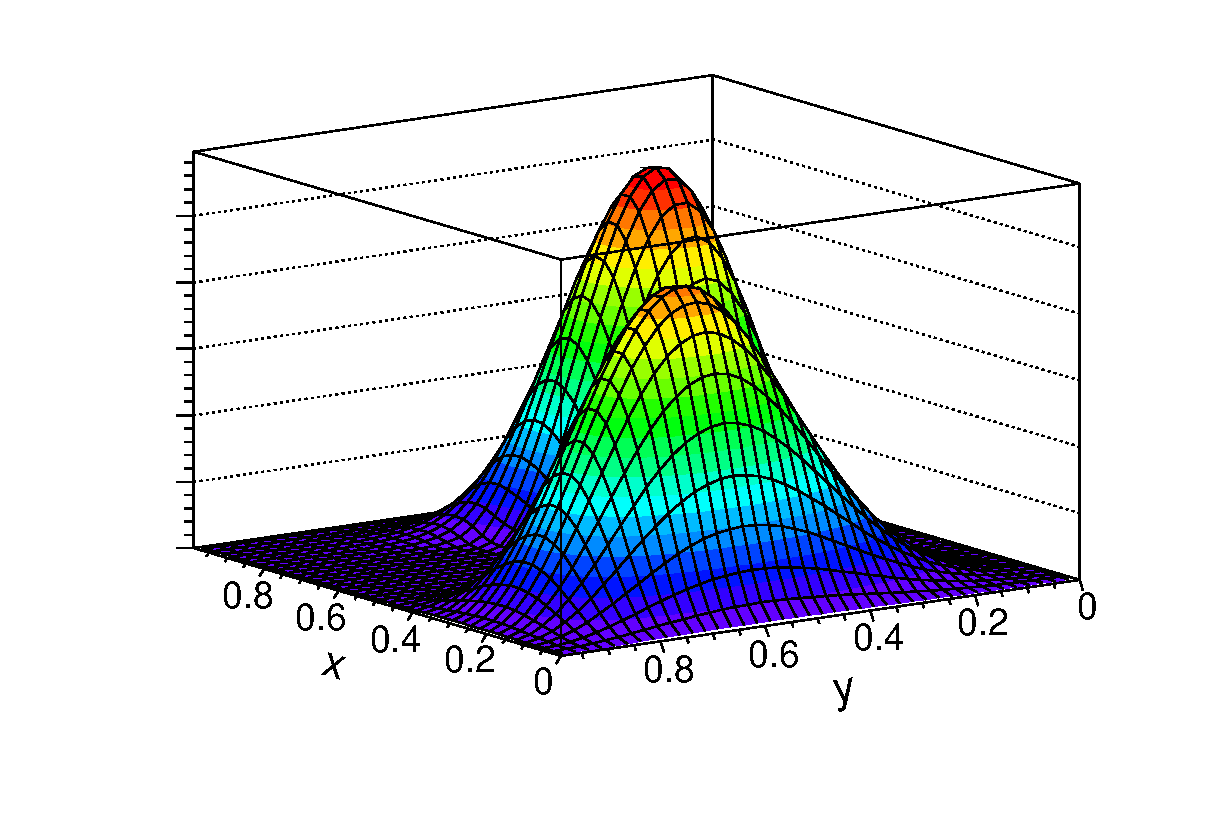
\includegraphics[width=0.5\textwidth]{figures/second2.eps}}\\
  \subfloat[][]{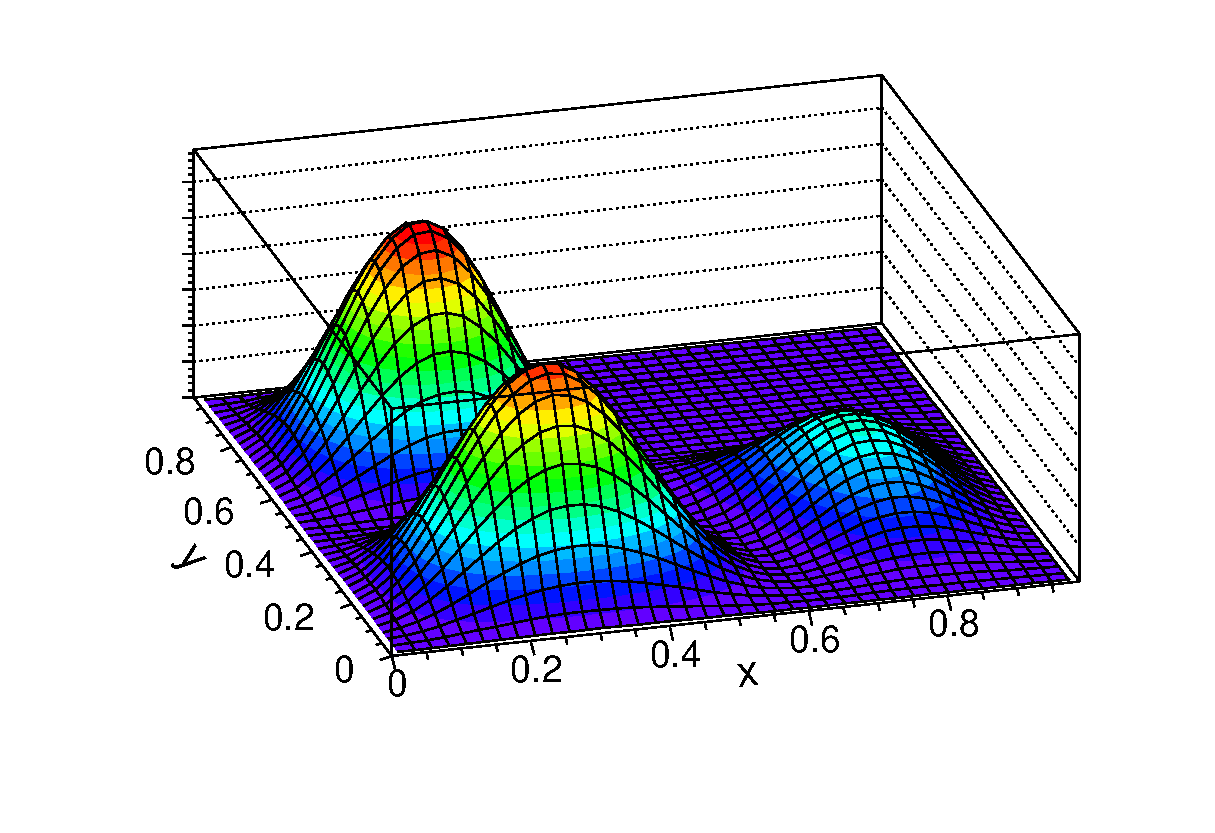
\includegraphics[width=0.5\textwidth]{figures/third1.eps}}
  \subfloat[][]{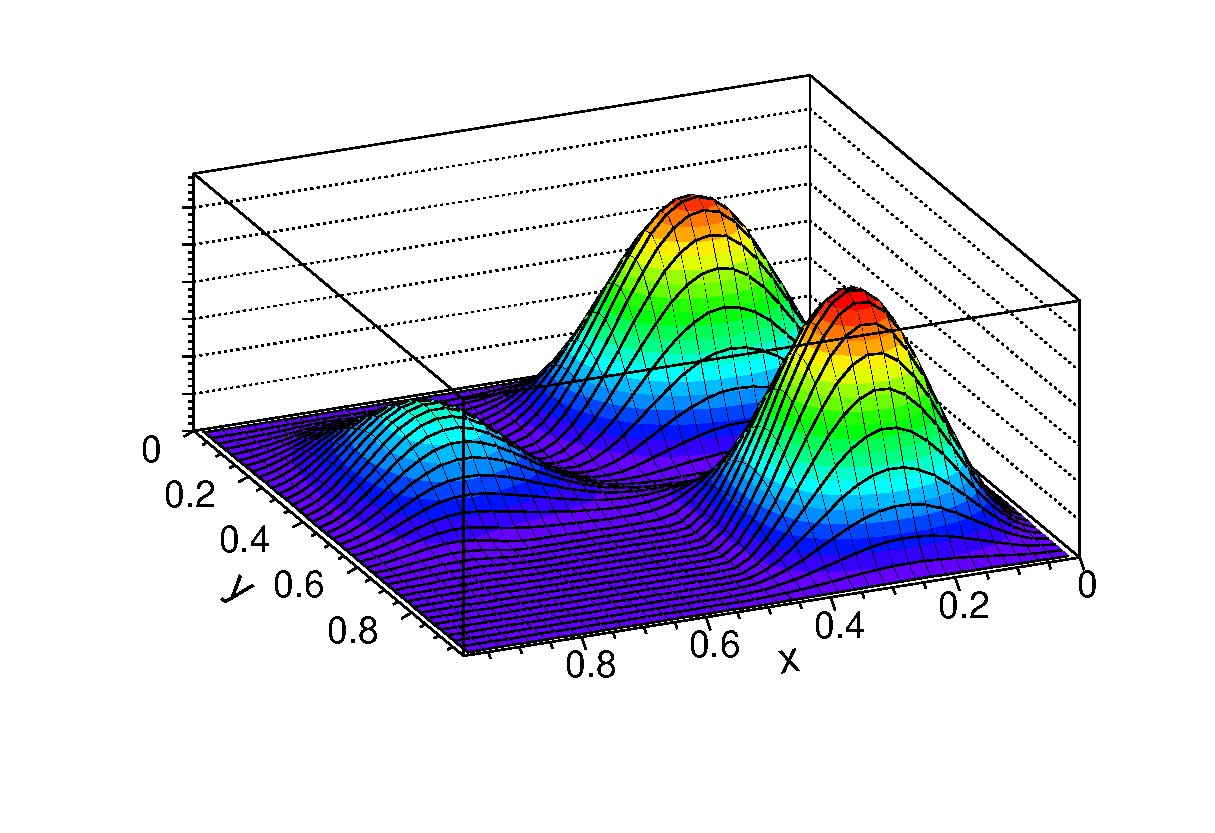
\includegraphics[width=0.5\textwidth]{figures/third3.eps}}\\
  \caption{\label{particles} ``SURF'' plots for three lowest eigenstates of particle in a box with infinite square. The probability ditribution avoids the infinite rectangle on corner as expected.}
\end{figure}

\clearpage
\section{Charged particle Schrodinger equation}


\end{document}
